\documentclass[a4paper, 12pt]{article}
%\usepackage{fontspec}
%\setmainfont{Times New Roman}
\usepackage{CJKutf8}
\usepackage{caption}
\usepackage[ruled,linesnumbered]{algorithm2e}
\usepackage{color}
\usepackage{indentfirst}
% \usepackage{natbib}
\usepackage{graphicx}
\usepackage{float}
\usepackage{amsmath}
% \let\Bbbk\relax %% fix bug
\usepackage{amssymb}
\usepackage{amsmath}
\usepackage{amstext}
\usepackage{amsopn}
\usepackage{graphicx}
\usepackage{textcomp}
\usepackage{xcolor}
\usepackage{textcomp}
\usepackage{boxedminipage}
\usepackage{enumerate}
\usepackage{url}
\usepackage{times}
% \usepackage[pdftex]{graphicx}
\usepackage{epsfig}
\usepackage{epsf}
%\usepackage{graphics}
\usepackage{caption}
\usepackage{subfigure}
\usepackage{algpseudocode}
%\PassOptionsToPackage{bookmarks={false}}{hyperref}
%%%%%%%%%%%%
\usepackage{placeins}
\usepackage{comment}
\usepackage{multicol}
\usepackage{booktabs}
\usepackage{dblfloatfix}
\usepackage{bm}
\usepackage{multicol}
\usepackage{hyperref}
% \usepackage{notoccite}
% \usepackage{soul}
% \usepackage{subfigure}
\linespread{1.5}
\setlength{\parindent}{2em}
\setlength{\hoffset}{0in}
\setlength{\voffset}{0in}
\setlength{\oddsidemargin}{0.05in}
\setlength{\evensidemargin}{0in}
\setlength{\topmargin}{0in}
\setlength{\headheight}{0.167in}
\setlength{\headsep}{0.333in}
\setlength{\textwidth}{6.268in}
\setlength{\textheight}{9.393in}
\setlength{\marginparsep}{0in}
\setlength{\marginparwidth}{0in}
\setlength{\marginparpush}{0in}
\setlength{\footskip}{0.5in}

% \setCJKmainfont{Noto Serif CJK SC}

\input lstset.tex
\input macro.tex

\begin{document}

\renewcommand{\abstractname}{\large 摘要}

\newcommand{\pluseq}{\mathrel{+}=}

\begin{CJK}{UTF8}{bkai}
	\captionsetup[figure]{labelfont={bf},name={圖},labelsep=period}
    \captionsetup[table]{name={表格},labelsep=period}
	\title{GAN 應用於黑白畫面上色 \& 畫面風格轉換}
	\author{B093040007 張碩文 \\ B092040016 陳昱逢}
	\date{}
	\maketitle
    \section{Motivation \& Features}
		\subsection{Motivation}
		作為一個喜愛 1950-60 年代音樂的愛好者,我發現當時的影像資料多為黑白錄像,像是 The Beatles 和 Chuck Berry 等演唱會錄像。由於當時攝影技術的限制,在 youtube 現存的錄像大多沒有彩色版本。為了讓這些影像整體的觀看感可更加逼真,本專案採用 GAN 生成對抗網絡模型去生成彩色影像,並轉換成各式各樣的藝術風格影片。
		\subsection{Features}
			\subsubsection{技術背景}
			\begin{enumerate}
				\item 本專案採用了 Conditional GAN(CGAN)\cite{pix2pix} 和 Cycle GAN \cite{cyclegan} 兩種生成對抗網絡模型。CGAN \cite{pix2pix}  用於將黑白影片自動上色,而 Cycle GAN \cite{cyclegan} 則將上色後的影片轉換成四種藝術風格:Monet、Van Gogh、Cezanne 和 Ukiyo-e
				\item CGAN \cite{pix2pix} 的理論參考自 Isola 等人於 2017 年 CVPR 發佈的論文《Image-to-Image Translation with Conditional Adversarial Networks》
				\item Cycle GAN \cite{cyclegan} 的理論參考自 Zhu 等人於 2017 年 CVPR 發佈的論文《Unpaired Image-to-Image Translation using Cycle-Consistent Adversarial Networks》 
			\end{enumerate}
			\subsubsection{技術挑戰}
			兩篇論文的方法實作細節均在 Github \cite{torch-cyclegan-pix2pix} 上有提供程式碼和相關的預訓練模型,然而將黑白影片上色的模型,未提供預訓練模型和訓練資料集,因此需自行收集資料後再使用提供的訓練模型之程式碼訓練,在本專案中,使用一張 RTX 3090 訓練仍需耗時 5 小時才訓練完成,在調整模型上會有大量的時間成本,且訓練資料集上雖蒐集了 4000 張圖片,但結果上仍有上色不穩定的情況發生。
			\subsubsection{本專案優勢}
			\begin{enumerate}
				\item 由於兩篇論文所提供的程式碼均有 yml 檔,因此在環境安裝時,可非常有效率地完成,執行程式也能避免版本不相容的問題。
				\item 直接使用 Github \cite{torch-cyclegan-pix2pix} 上現有程式碼進行修改,節省開發時間。
			\end{enumerate}
    \section{Method}
		\subsection{Overall architecture \& Data Preprocessing}

			\begin{figure}[tbh]
				\centering
				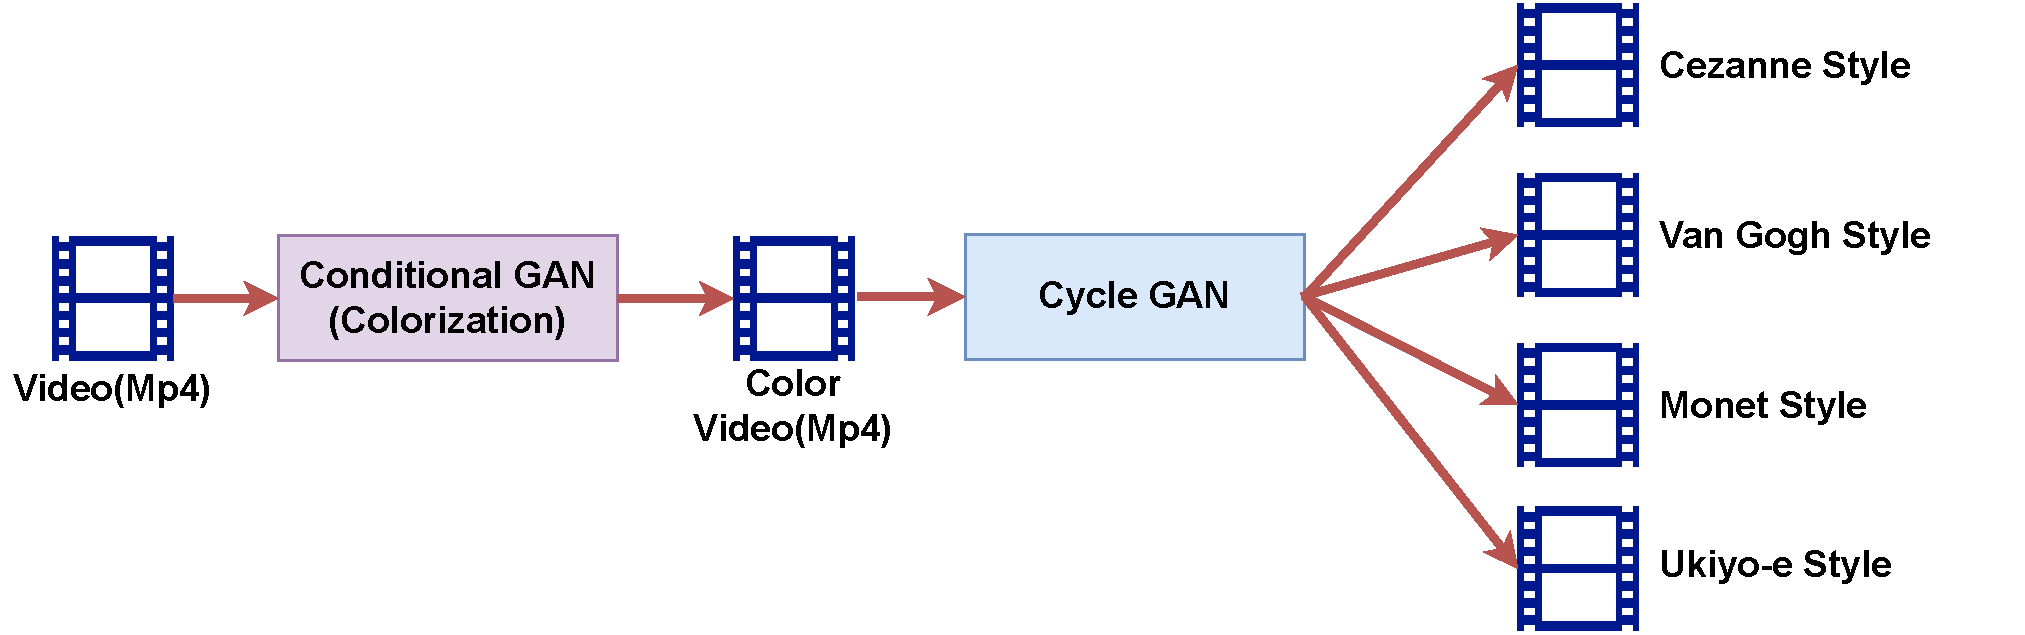
\includegraphics[width=0.8\textwidth]{src/Overall_Architecture.pdf}
				\caption{架構圖}
				\label{fig-Overall_Architecture}
			\end{figure}
			
			該架構圖共可分為兩大部分,把黑白影片上色用的 Conditional GAN (Colorization) \cite{pix2pix},以及風格轉換用的 Cycle GAN \cite{cyclegan},在原始影片進入模型前需經過三個前處理步驟。
			\begin{enumerate}
				\item 圖片 resize 成 $(286, 286)$
				\item 使用 Crop 擷取中間的區塊變成 $(256, 256)$
				\item 轉乘 Lab 的形式,並拆成 L 和 ab 兩個部分
			\end{enumerate}
			其中 Lab 的 $L$ 代表該圖片的亮度,$a$ 代表紅綠軸上的的座標,$b$ 代表黃藍軸上的座標。
			最後僅有 L 通道的圖片(灰階圖),其 shape 為 $(1, 256, 256)$,輸入到 Colorization model 轉成彩色圖片後,再使用 Cycle GAN 轉成 Monet、Van Gogh、Cezanne 和 Ukiyo-e 四種風格的影片。
			
		\subsection{Conditional GAN (CGAN)}
			\begin{figure}[tbh]
				\centering
				\includegraphics[width=0.8\textwidth]{src/CGAN.png}
				\caption{Conditional GAN 內部架構圖 \cite{hungyiML}}
				\label{fig-CGAN}
			\end{figure}
			如\xfig{fig-CGAN}所示,Conditional GAN 內部可分為兩個部分,$G$ (Generator) 和 $D$ (Discrminator),該模型需成對的資料集進行訓練,其中 $G$ 的輸入為一張灰階的圖 $x$ 和隨機從已知的機率分布中隨機抽取出的向量 $Z$,且這邊的灰階圖可直接視為條件輸入,$G$ 的輸出為一張彩圖 $G(x, z)$,這時 $D$ 會同時接收 Generator 產生的彩圖和原始圖片的彩圖,再去分辨哪張彩圖是原始圖片,若分類結果越準,輸出的 scalar 值會越大,該 scalar 的計算方式如下式:
			\begin{equation}
				\mathcal{L}_{cGAN}(G,D) = E_{x,y}\left[ logD(x,y) \right] + E_{x,z}\left[ log(1 - D(x,G(x,z))) \right]
			\end{equation}
			此模型其最佳化目標為找到一組 $G$ 和 $D$,$D$ 要最大化 scalar 的值,同時 $G$ 要最小化 $D$ 所產生的 scalar,其目標函數如下式:
			\begin{equation}
				\arg \min_G \max_D \mathcal{L}_{\text{cGAN}}(G, D)
			\end{equation}
			\subsubsection{Generator Architecture}
			\begin{enumerate}
				\item Input Layer,其中 Input shape $(1, 256, 256)$  (L 通道)
				\item 8 層 downsampler
				\item 8 層 upsampler
				\item Output Layer,其中 Output shape $(2, 256, 256)$ (ab 通道)
			\end{enumerate}

			\subsubsection{Discrminator Architecture}
			\begin{enumerate}
				\item 1 層 Input Layer (Conv2D),其中 Input shape $(3, 256, 256)$ 的 Lab 圖片
				\item 3 層 Intermediate Layer (Conv2D)
				\item 1 層 Output Layer (Conv2D),其中 Output shape 是一個 scalar ,分數越高,代表 Discrminator 越強
			\end{enumerate}


			
		\subsection{Cycle GAN}
		
		\begin{figure}[tbh]
			\centering
			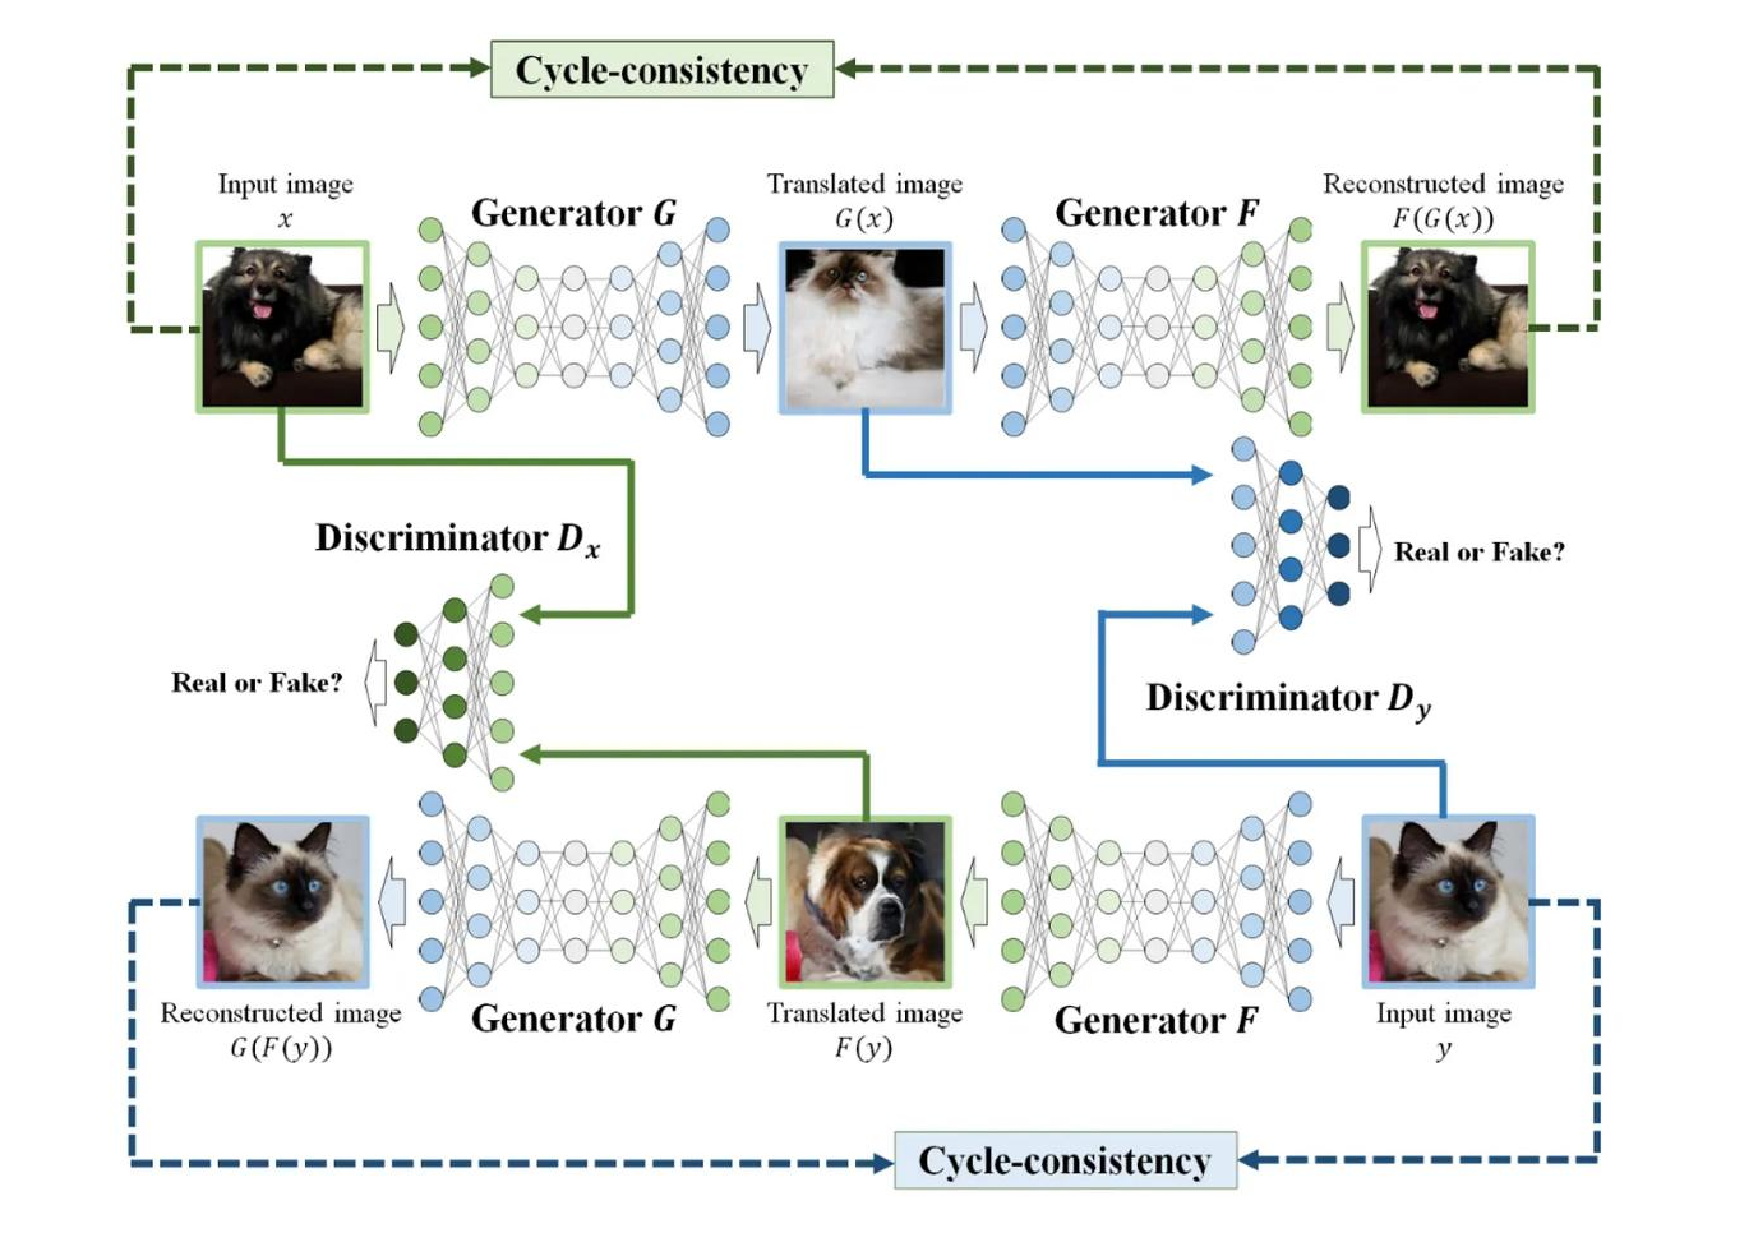
\includegraphics[width=0.65\textwidth]{src/cyclegan.pdf}
			\caption{Cycle GAN 內部架構圖 \cite{medium}}
			\label{fig-CycleGAN_Architecture}
		\end{figure}
		\xfig{fig-CycleGAN_Architecture}展示 Cycle GAN 方法, 主要用於不對稱的資料集訓練,因此可進行風格轉換等任務,Cycle GAN 有兩個 Generator 兩個 Discrminator,訓練中加入了 Consistency loss,主要希望將照片經過兩個 Generator 轉換後,能夠達成重建影像的目的。整個 Cycle GAN 的學習目標如下式:
		
		\begin{equation}
			\begin{aligned}
			\mathcal{L}_{\text{CycleGAN}}(G, F, D_x, D_y) = &
			\mathbb{E}_{y \sim p_{\text{data}}(y)} \left[ \log D_y(y) \right] + \mathbb{E}_{x \sim p_{\text{data}}(x)} \left[ \log (1 - D_y(G(x))) \right] \\
			&+ \mathbb{E}_{x \sim p_{\text{data}}(x)} \left[ \log D_x(x) \right] + \mathbb{E}_{y \sim p_{\text{data}}(y)} \left[ \log (1 - D_x(F(y))) \right] \\
			&+ \lambda_{\text{cyc}(x)} \mathbb{E}_{x \sim p_{\text{data}}(x)} \left[ \| F(G(x)) - x \|_1 \right] \\
			&+ \lambda_{\text{cyc}(y)} \mathbb{E}_{y \sim p_{\text{data}}(y)} \left[ \| G(F(y)) - y \|_1 \right],
			\end{aligned}
		\end{equation}
			
		
		跟一般 GAN 的 Generator 使用 U-Net 不一樣的是,其 Generator 是基於 ResNet 架構,原因為 U-Net 比較適合用在成對的資料集上,因為 U-Net 中的 skip connection 會把每一層取到的特徵在後面結合起來。但對於不成對的資料集問題,我們需要將一個分佈的資料,根據其特徵以及輪廓,轉換到另一目標分佈的資料上,因此採用 ResNet 在萃取特徵上表現較好。在實作細節中,Cycle GAN 使用 LSGAN \cite{lsgan} 的損失函數代替了 negative log liklihood,也加入了 Identity Loss 等技巧。
		
	\section{Experimental Results}

	\subsection{資料收集}

	訓練資料收集了 4000 張圖片,其中 3400 張來自 MS COCO \cite{mscoco},600 張來自 \cite{lab2rgb},且皆是隨機挑選,驗證集收集 75 張圖片 \cite{lab2rgb}。 測試機收集了四部影片,其中 Beatles 一部,卓別林兩部,道路縮時攝影一部。
	



	\subsection{Experimental Results}

	完整 demo 影片已存放至:
	\href{https://drive.google.com/drive/folders/1SVA7trdCwTGiufNew1d3kUPHCUO1aqrz?usp=drive_link}{Demo Video Link}

    \section{Conclusion \& Future work}

	本專案結合了 Conditional GAN 以及 Cycle GAN 來完成黑白影像上色以及轉換成其他藝術風格。我們在訓練 Colorization model 時都是給定圖片資料集,可能對於連續影像的上色會有色塊不連續的問題,視覺上有不協調性,那也會影響後續的風格轉換的結果。
	由實驗結果可以看出,對於背景屬於靜態的畫面時,自動上色的結果較好,而風格轉換時,對於有藝術品的特徵時,表現較好。

    \bibliographystyle{IEEEtran}
    \bibliography{reference} 
    
\end{CJK}

\end{document}